\documentclass{standalone}
\usepackage{graphicx}	
\usepackage{amssymb, amsmath, amsthm}
\usepackage{color}

\usepackage{tikz}
\usetikzlibrary{intersections, backgrounds, math}

\definecolor{light}{RGB}{220, 188, 188}
\definecolor{mid}{RGB}{185, 124, 124}
\definecolor{dark}{RGB}{143, 39, 39}
\definecolor{highlight}{RGB}{180, 31, 180}
\definecolor{darkteal}{RGB}{29, 79, 79}
\definecolor{darkolive}{RGB}{97, 123, 45}
\definecolor{gray10}{gray}{0.1}
\definecolor{gray20}{gray}{0.2}
\definecolor{gray30}{gray}{0.3}
\definecolor{gray40}{gray}{0.4}
\definecolor{gray60}{gray}{0.6}
\definecolor{gray70}{gray}{0.7}
\definecolor{gray80}{gray}{0.8}
\definecolor{gray90}{gray}{0.9}
\definecolor{gray95}{gray}{0.95}

\begin{document}

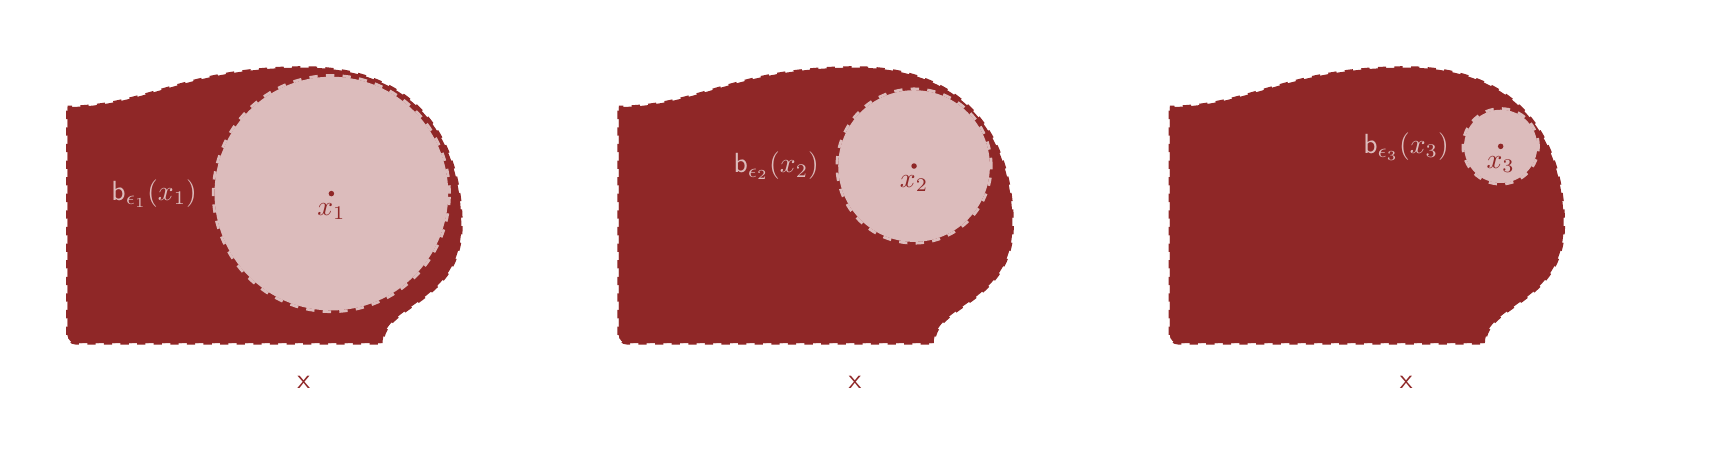
\begin{tikzpicture}[scale=1.0]
  
  \begin{scope}[shift={(0, 0)}]
    \draw[white] (-3.5, -3) rectangle (3.5, 2);
  
    \begin{scope}
      \clip (-3.5, -3) rectangle (1, 1);
      \draw[rounded corners=3, dark, dashed, line width=1] (-3, -2) rectangle (3, 2);
    \end{scope}
    
    \begin{scope}
      \clip[rounded corners=3] (-3, -2) rectangle (3, 2);
      \fill[dark, line width=1] (-3, -2) --
                                (-3, 1) .. controls (-2, 1) and (-1.5, 1.5) .. 
                                (0, 1.5) .. controls (1.5, 1.5) and (2, 0.5) .. 
                                (2, -0.5) .. controls (2, -1.5) and (1, -1.5) .. 
                                (1, -2) -- cycle;
      \draw[dark, line width=1, dashed] (-3, -2) --
                          (-3, 1) .. controls (-2, 1) and (-1.5, 1.5) .. 
                          (0, 1.5) .. controls (1.5, 1.5) and (2, 0.5) .. 
                          (2, -0.5) .. controls (2, -1.5) and (1, -1.5) .. 
                          (1, -2) -- cycle;
    \end{scope}
    
    \draw[light, dashed, line width=1] (0.35, -0.1) circle (1.5);
    \fill[light] (0.35, -0.1) circle (1.484);
    \node[light] at (-1.9, -0.1) { $\mathsf{b}_{\epsilon_{1}}(x_{1})$ };
    \fill[dark] (0.35, -0.1) circle (0.035) node[below, dark] { $x_{1}$ };

    \node[dark] at (0, -2.5) { $\mathsf{x}$ };
  \end{scope}
  
  \begin{scope}[shift={(7, 0)}]
    \draw[white] (-3.5, -3) rectangle (3.5, 2);
  
    \begin{scope}
      \clip (-3.5, -3) rectangle (1, 1);
      \draw[rounded corners=3, dark, dashed, line width=1] (-3, -2) rectangle (3, 2);
    \end{scope}
    
    \begin{scope}
      \clip[rounded corners=3] (-3, -2) rectangle (3, 2);
      \fill[dark, line width=1] (-3, -2) --
                                (-3, 1) .. controls (-2, 1) and (-1.5, 1.5) .. 
                                (0, 1.5) .. controls (1.5, 1.5) and (2, 0.5) .. 
                                (2, -0.5) .. controls (2, -1.5) and (1, -1.5) .. 
                                (1, -2) -- cycle;
      \draw[dark, line width=1, dashed] (-3, -2) --
                    (-3, 1) .. controls (-2, 1) and (-1.5, 1.5) .. 
                    (0, 1.5) .. controls (1.5, 1.5) and (2, 0.5) .. 
                    (2, -0.5) .. controls (2, -1.5) and (1, -1.5) .. 
                    (1, -2) -- cycle;
    \end{scope}
    
    \draw[light, dashed, line width=1] (0.75, 0.25) circle (0.98);
    \fill[light] (0.75, 0.25) circle (0.963);
    \node[light] at (-1, 0.25) { $\mathsf{b}_{\epsilon_{2}}(x_{2})$ };
    \fill[dark] (0.75, 0.25) circle (0.035) node[below, dark] { $x_{2}$ };
    
    \node[dark] at (0, -2.5) { $\mathsf{x}$ };
  \end{scope}
  
  \begin{scope}[shift={(14, 0)}]
    \draw[white] (-3.5, -3) rectangle (3.5, 2);
  
    \begin{scope}
      \clip (-3.5, -3) rectangle (1, 1);
      \draw[rounded corners=3, dark, dashed, line width=1] (-3, -2) rectangle (3, 2);
    \end{scope}
    
    \begin{scope}
      \clip[rounded corners=3] (-3, -2) rectangle (3, 2);
      \fill[dark, line width=1] (-3, -2) --
                                (-3, 1) .. controls (-2, 1) and (-1.5, 1.5) .. 
                                (0, 1.5) .. controls (1.5, 1.5) and (2, 0.5) .. 
                                (2, -0.5) .. controls (2, -1.5) and (1, -1.5) .. 
                                (1, -2) -- cycle;
      \draw[dark, line width=1, dashed] (-3, -2) --
                          (-3, 1) .. controls (-2, 1) and (-1.5, 1.5) .. 
                          (0, 1.5) .. controls (1.5, 1.5) and (2, 0.5) .. 
                          (2, -0.5) .. controls (2, -1.5) and (1, -1.5) .. 
                          (1, -2) -- cycle;
    \end{scope}
    
    \draw[light, dashed, line width=1] (1.2, 0.5) circle (0.48);
    \fill[light] (1.2, 0.5) circle (0.465);
    \node[light] at (0, 0.5) { $\mathsf{b}_{\epsilon_{3}}(x_{3})$ };
    \fill[dark] (1.2, 0.5) circle (0.035) node[below, dark] { $x_{3}$ };
    
    \node[dark] at (0, -2.5) { $\mathsf{x}$ };
  \end{scope}
  
\end{tikzpicture}

\end{document}  